\documentclass{article}\usepackage[]{graphicx}\usepackage[]{color}
%% maxwidth is the original width if it is less than linewidth
%% otherwise use linewidth (to make sure the graphics do not exceed the margin)
\makeatletter
\def\maxwidth{ %
  \ifdim\Gin@nat@width>\linewidth
    \linewidth
  \else
    \Gin@nat@width
  \fi
}
\makeatother

\definecolor{fgcolor}{rgb}{0.345, 0.345, 0.345}
\newcommand{\hlnum}[1]{\textcolor[rgb]{0.686,0.059,0.569}{#1}}%
\newcommand{\hlstr}[1]{\textcolor[rgb]{0.192,0.494,0.8}{#1}}%
\newcommand{\hlcom}[1]{\textcolor[rgb]{0.678,0.584,0.686}{\textit{#1}}}%
\newcommand{\hlopt}[1]{\textcolor[rgb]{0,0,0}{#1}}%
\newcommand{\hlstd}[1]{\textcolor[rgb]{0.345,0.345,0.345}{#1}}%
\newcommand{\hlkwa}[1]{\textcolor[rgb]{0.161,0.373,0.58}{\textbf{#1}}}%
\newcommand{\hlkwb}[1]{\textcolor[rgb]{0.69,0.353,0.396}{#1}}%
\newcommand{\hlkwc}[1]{\textcolor[rgb]{0.333,0.667,0.333}{#1}}%
\newcommand{\hlkwd}[1]{\textcolor[rgb]{0.737,0.353,0.396}{\textbf{#1}}}%
\let\hlipl\hlkwb

\usepackage{framed}
\makeatletter
\newenvironment{kframe}{%
 \def\at@end@of@kframe{}%
 \ifinner\ifhmode%
  \def\at@end@of@kframe{\end{minipage}}%
  \begin{minipage}{\columnwidth}%
 \fi\fi%
 \def\FrameCommand##1{\hskip\@totalleftmargin \hskip-\fboxsep
 \colorbox{shadecolor}{##1}\hskip-\fboxsep
     % There is no \\@totalrightmargin, so:
     \hskip-\linewidth \hskip-\@totalleftmargin \hskip\columnwidth}%
 \MakeFramed {\advance\hsize-\width
   \@totalleftmargin\z@ \linewidth\hsize
   \@setminipage}}%
 {\par\unskip\endMakeFramed%
 \at@end@of@kframe}
\makeatother

\definecolor{shadecolor}{rgb}{.97, .97, .97}
\definecolor{messagecolor}{rgb}{0, 0, 0}
\definecolor{warningcolor}{rgb}{1, 0, 1}
\definecolor{errorcolor}{rgb}{1, 0, 0}
\newenvironment{knitrout}{}{} % an empty environment to be redefined in TeX

\usepackage{alltt}
\usepackage{natbib}
\IfFileExists{upquote.sty}{\usepackage{upquote}}{}
\begin{document}



\title{H.P. Lovecraft Word cloud}
\author{Kimberly Staudt}
\maketitle

\begin{abstract}
In this article, we create a word cloud using tidytext and gutenbergr,for H.P. Lovecraft's novel, \textit{The Dunwich Horror}. 
\end{abstract}

\noindent This 1929 horror classic follows the peculiar Wilbur Whateley,and his wizard grandfather who create a monster.This world cloud is constructed of the most frequently used words in the novel.

\section{Packages and Filtering}
To begin install the following packages: tidytext, tm, wordcloud, gutenbergr, and stringr. Dplyr comes with tidytext, so pull this from the library as seen below. To find the novel's ID, filter the title. This can apply to any novel within gutenbergr.Once the ID number is found, download and store into the data frame, Horror. 

\begin{knitrout}
\definecolor{shadecolor}{rgb}{0.969, 0.969, 0.969}\color{fgcolor}\begin{kframe}
\begin{alltt}
\hlkwd{library}\hlstd{(tidytext)}
\hlkwd{library}\hlstd{(dplyr)}
\hlkwd{library}\hlstd{(gutenbergr)}

\hlstd{Dunwich}\hlkwb{<-}\hlkwd{gutenberg_works}\hlstd{()} \hlopt
  \hlkwd{filter}\hlstd{(title} \hlopt{==} \hlstr{"The Dunwich Horror"}\hlstd{)}

\hlstd{Horror}\hlkwb{<-}\hlkwd{gutenberg_download}\hlstd{(}\hlnum{50133}\hlstd{)}
\end{alltt}
\end{kframe}
\end{knitrout}

\noindent Next, us the string detect function to filter and remove text with the word CHAPTER. 
\begin{knitrout}
\definecolor{shadecolor}{rgb}{0.969, 0.969, 0.969}\color{fgcolor}\begin{kframe}
\begin{alltt}
\hlkwd{library}\hlstd{(stringr)}
\hlstd{Horror}\hlkwb{<-}\hlstd{Horror}\hlopt
  \hlkwd{filter}\hlstd{(}\hlopt{!}\hlkwd{str_detect}\hlstd{(Horror}\hlopt{$}\hlstd{text,}\hlstr{'CHAPTER'}\hlstd{))}
\end{alltt}
\end{kframe}
\end{knitrout}

\section{Create a New Column}
\noindent Unnest the text to create a new column, word. Stop words are common language, such as articles or pronouns, that would be overly present in text. We are trying to isolate unique language that separates the novel from others by eliminating these with the "!" character. Store this data into a new data frame.
\begin{knitrout}
\definecolor{shadecolor}{rgb}{0.969, 0.969, 0.969}\color{fgcolor}\begin{kframe}
\begin{alltt}
\hlstd{words_df}\hlkwb{<-}\hlstd{Horror}\hlopt
  \hlkwd{unnest_tokens}\hlstd{(word,text)}

\hlstd{words_df}\hlkwb{<-}\hlstd{words_df}\hlopt
  \hlkwd{filter}\hlstd{(}\hlopt{!}\hlstd{word} \hlopt \hlstd{stop_words}\hlopt{$}\hlstd{word)}
\end{alltt}
\end{kframe}
\end{knitrout}

\noindent To find the frequency of the words, group the data by word and use count to summarize how many times this word appears. Store into a new data frame.
\begin{knitrout}
\definecolor{shadecolor}{rgb}{0.969, 0.969, 0.969}\color{fgcolor}\begin{kframe}
\begin{alltt}
\hlstd{word_freq}\hlkwb{<-}\hlstd{words_df}\hlopt
  \hlkwd{group_by}\hlstd{(word)}\hlopt
  \hlkwd{summarise}\hlstd{(}\hlkwc{count}\hlstd{=}\hlkwd{n}\hlstd{())}
\end{alltt}
\end{kframe}
\end{knitrout}

\section{Visualization}
\noindent Now we can create our word cloud by using the word frequency data frame. The freq function allows you to adjust the size of the cloud. By using a frequency of 10, words appear 10 times in the text before they are displayed in the cloud. The higher the number, the smaller the word cloud. RColorBrewer allows you to choose the color pallete of your desire, but in this example our word cloud will be black.
\begin{knitrout}
\definecolor{shadecolor}{rgb}{0.969, 0.969, 0.969}\color{fgcolor}\begin{kframe}
\begin{alltt}
\hlkwd{library}\hlstd{(wordcloud)}
\hlkwd{wordcloud}\hlstd{(word_freq}\hlopt{$}\hlstd{word,word_freq}\hlopt{$}\hlstd{count,}\hlkwc{min.freq}\hlstd{=}\hlnum{10}\hlstd{)}
\end{alltt}
\end{kframe}
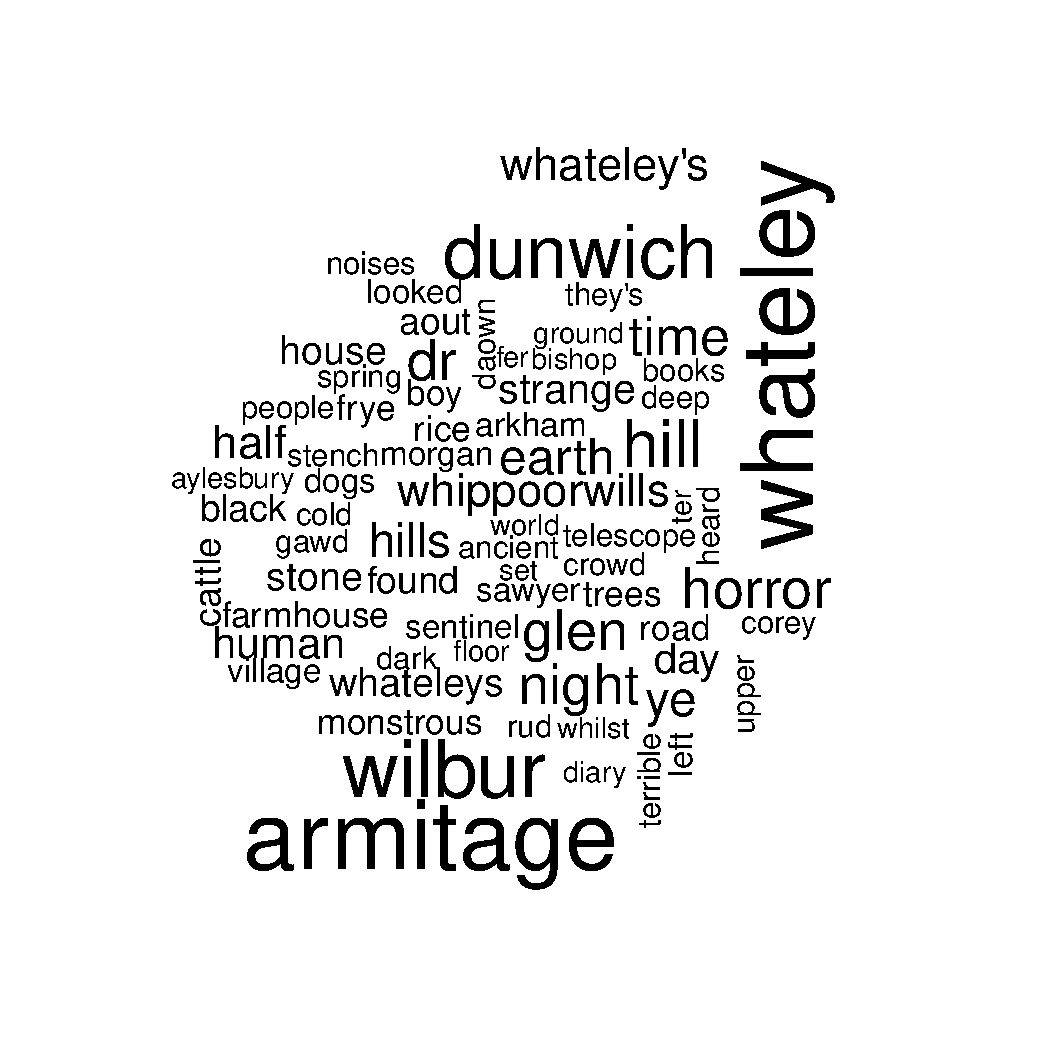
\includegraphics[width=\maxwidth]{figure/unnamed-chunk-6-1} 

\end{knitrout}

\bibliographystyle{apa}
\bibliography{article,packages}
\nocite{*}


\end{document}
